\documentclass[11pt, oneside]{report}  %can try book instead    % use "amsart" instead of "article" for AMSLaTeX format
\usepackage[margin = 0.7in, bmargin = 1.1in, tmargin = 0.9in]{geometry}                     % See geometry.pdf to learn the layout options. There are lots.
\geometry{a4paper}                          % ... or a4paper or a5paper or ... 
%\geometry{landscape}                       % Activate for rotated page geometry
\usepackage[parfill]{parskip}           % Activate to begin paragraphs with an empty line rather than an indent
\usepackage{graphicx}               % Use pdf, png, jpg, or eps§ with pdflatex; use eps in DVI mode
                                % TeX will automatically convert eps --> pdf in pdflatex        
\usepackage{amssymb}
\usepackage{amsmath}
\usepackage{amsmath,mathtools}
\usepackage{array}
\usepackage{tabu}
\usepackage{bm}
\usepackage{wrapfig}
\usepackage{multirow}
\usepackage{physics}
\usepackage{hyperref}
\usepackage{listings}
\usepackage[utf8]{inputenc}
\usepackage[T1]{fontenc}
\usepackage{lmodern}
%\usepackage{graphicx} %already declared above
\usepackage{caption}
\usepackage{float}
\usepackage{floatrow}
\usepackage{subfig}
\usepackage{multicol}
\usepackage{xcolor}
\usepackage{pagecolor}
\usepackage{lipsum}  
\usepackage{mdframed}
\usepackage{verbatim}
\usepackage{slashed}
%\usepackage[compat=1.1.0]{tikz-feynman}
%\usepackage{animate}


\newcommand{\G}{\mathcal{G}}
\newcommand{\D}{\mathcal{D}}
\newcommand{\E}{\mathcal{E}}
\renewcommand{\S}{\mathcal{S}}
\newcommand{\M}{\mathcal{M}}
\newcommand{\K}{\mathcal{K}}
\renewcommand{\L}{\mathcal{L}}
\newcommand{\R}{\mathcal{R}}
\renewcommand{\P}{\mathcal{P}}
\newcommand{\vp}{\varphi}
\newcommand{\T}{\mathcal{T}}
\newcommand{\A}{\mathcal{A}}
\newcommand{\bs}{\boldsymbol}
\newcommand{\rspace}{\mathbb{R}}
\newcommand{\dd}{\mathrm{d}}


\definecolor{purple}{RGB}{38,0,75}
\pagecolor{white}
\color{black}

%SetFonts

%SetFonts
\usepackage{subfiles} % Best loaded last in the preamble

\numberwithin{equation}{section}
\pagenumbering{gobble}
\title{Third Term Report}
\author{Robin Croft}
%\date{}    
\begin{document}







%\newpage
%\pagenumbering{arabic}
\tableofcontents
\newpage


\section{Introduction}
general gr shit?
mention einstein derivation (hilbert derivation a potentially earlier but vacuum), karl schwarzshild ( ironicaly meaning black shield), then low mass limit, photon deflection and mercury perihelion around sun. mention cosmology, gravitational waves, more black holes, minkowski. more compact objects. 

\section{Introduction to Compact Objects and Boson Stars}
The first non-trivial solution to Einstein's equation found was that of the spherically symmetric, static and asymptotically flat vacuum spacetime by Karl Schwarzschild in 1915. The solution was designed to be used outside a spherically symmetric, non-spinning, body of mass; however it turned out to provide use in describing black holes. This metric was then modified by Tolman, Oppenheimer and Volkov in 1939 to describe the non-vacuum case of a constant density neutron star. This turned out to give an unphysical estimate of $0.7 M_\odot$ for the upper limit of neutron star mass due to the equation of state. 

The study of compact exotic objects can be traced back to John Wheeler who investigated Geons in 1955 for their potential similarity to elementary particles. Geons are gravito-electromagnetic objects with the name arising from "gravitational electromagnetic entity". In 1968 David Kaup published [] describing what he called "Klein-Gordon Geons", nowadays referred to as boson stars. Importantly, boson stars are a localised complex Klein-Gordon configuration, with the real counterparts being unstable. Many variants such as (Spin 1) proca stars [], electromagnetically charged boson stars and many others have been studied. 

Interest in boson stars remains for many reasons. Given the recent discovery of the higgs boson, we know that scalar fields exist in nature and any gravitational wave signals created by compact objects could theoretically be detected with modern gravitational wave interferometers. Secondly, boson stars are a good candidate for dark matter haloes. Boson stars are also useful as a proxy to other compact objects in general relativity; there is a lot of freedom in the construction of different types of boson star and they can be fine tuned to model dense neutron stars for one example. The advantage this would have over simulating a real fluid is that the Klein Gordon equation is linear in the principal part meaning smooth data must always remain smooth; thus avoiding shocks and conserving particle numbers relatively well with less sophisticated numerical schemes. 

On a slightly different topic, collisions of boson stars could be a natural method to produce scalar hair around black holes which will be discussed later in more detail. 

\subsection{Conventions}
Throughout this thesis physical quantities will be expressed as a dimensionless ratio of the Planck length, time and mass $L_{pl}$, $T_{pl}$ and $M_{pl}$ respectively; consequently the constants $c$, $G$ and $\hbar$ evaluate numerically to $1$. As an example, Newtons equation of gravity would be recast like
\begin{equation}
F = \frac{G M m}{r^2} \rightarrow \left(\frac{F}{F_{pl}} \right)=\frac{\left(\frac{M}{M_{pl}} \right)\left(\frac{m}{M_{pl}} \right)  }{\left(\frac{r}{L_{pl}} \right)^2}
\end{equation}
where $F_{pl} = M_{pl}L_{pl}T_{pl}^{-2}$ is the Planck force.
$c=G=\hbar=1$, unless stated otherwise. The metric signature will always be $(-,+,+,+)$. 

Tensor fields will be denoted using bold font for
index free notation and normal font for the components.
The dot product between two vector fields will be written interchangeably as $\bs{A} \cdot \bs{B} \leftrightarrow {A}_\mu {B}^\mu$ for readability.
Additionally, $\nabla_\mu$ denotes the covariant derivative and $\partial_\mu$
is the partial derivative, both with respect to coordinate $x^\mu$.

When considering the ADM decomposition, as in [REF SECT], objects can be associated with both the $3+1$ dimensional manifold $\M$ or the $3$ dimensional hypersurface $\Sigma$. To differentiate here, standard Roman letters such as $R$ represent the object belonging to $\M$ and calligraphic letters such as $\mathcal{R}$ correspond to the projected object belonging to $\Sigma$. [MAYBE JUST REMOVE THIS BIT AND MAKE IT OBVIOUS IN THE ACTUAL 3+1 SECTION].

Finally, unless stated otherwise, Greek indices such
as $\{\alpha, \beta, ..., \mu, \nu, ...\}$ label four dimensional tensor components whereas late Latin indices such as $\{i, j, k, ...\}$ label
three dimensional tensor components and early Latin indices such as $\{a, b, ...\}$ label two dimensional ones. When the index range is unspecified and unimportant Greek letters will also be used.

make explicit th inner product, dot product, outer product (otimes) and wedge product (for forms, antisymm)






\section{Differential Geometry}
\subsection{Introduction to Geometry and Manifolds}
\begin{wrapfigure}{r}{0.45\textwidth}
\centering
    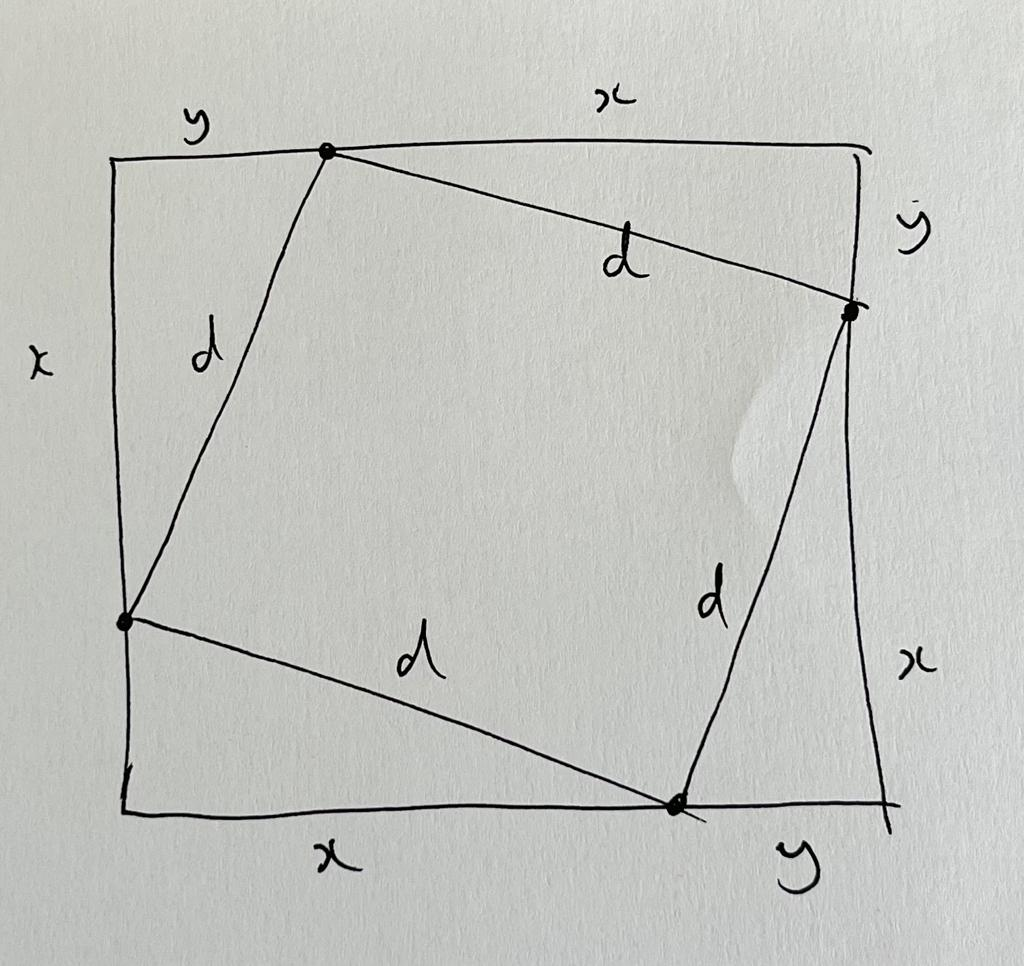
\includegraphics[width=0.45\textwidth]{pics/pythag_proof.png}
    \caption{Diagram for proof of Pythagoras' theorem.}
    \label{fig:pythag_proof}
\end{wrapfigure}




Everyones first encounter with geometry will cover Pythagoras' theorem; arguably the most famous and useful equation in existance. Pythagoras' equation relates the sidelengths of a right angled triangle, it says that $s^2 = x^2 + y^2$ for a triangle with height $y$, width $x$ and hypotenuse length $s$. This can be shown very simply by looking at Fig.~\ref{fig:pythag_proof}. The area of the partially rotated square is obviously $s^2$, but we can also calculate it from the the area of the larger square $A_{sq}$ and subtracting four times the area of one of the triangles $A_{tr}$. Clearly $A_{sq} = (x+y)^2$ and $A_{tr} = \frac{1}{2}xy$, therefore 
\begin{equation}
s^2 = (x+y)^2-2xy = x^2 + y^2
\end{equation}
and we have proved Pythagoras' theorem. Using an infinitessimally small triangle, we can write $\dd s^2 = \dd x^2 + \dd y^2$ and this can be trivially extended to arbitrary dimensions like
\begin{equation}\label{eq:pythag_inf}
\dd s^2 = \dd x^2 + \dd y^2 + \dd z^2 + ...\,\,\,.
\end{equation}
The infinitessimal form of Pythagoras' theorem is very powerful as it lets us calculate the length of a generic curve by approximating the curve as a collection of infinitessimally small straight lines with length $\dd s$. So far we have assumed that space is flat meaning Eq.~(\ref{eq:pythag_inf}) is true for all points in space, this is an assumpion we will have to drop if we want to study the curved spaces arising in strong gravity. In the next sections we will explore the generalisation of Pythagoras' equation to curved spaces and use it to measure curve lengths answell as volumes and areas. [REWRITE THIS WHEN THE SECTIONS ARE COMPLETE AND REF]

Differential Geometry (DG) is the extension of calculus, linear algebra and multilinear algebra to general
geometries. Einstein’s Theory of Relativity is written using the language of DG as it is the natural
way to deal with curves, tensor calculus and differential tensor equations in curved spaces. For a basic
introduction to DG, we should start with a manifold $\M$ which is an $N$ dimensional space that locally looks
like $\rspace^N$, $N$ dimensional Euclidean space. This is important as at a point $p\in\M$ we can find infinitesimally
close neighbouring points $p + \delta p \in \M$. In the following sections we will explore curves, functions, tensors and calculus on manifolds using DG.

\subsection{Functions, Curves and Tensors on Manifolds}
A real scalar function $f$ over $\M$ maps any point $p\in \M$ to a real number, this is denoted as
$f : p \rightarrow \rspace$. An important example of a set of scalar functions is the coordinate system $\phi$, $\phi : p \rightarrow \rspace^N$,
this is normally written $x^\mu$ where $\mu\in\{0,1,...,N-1\}$ is an index labelling the coordinate. The map $\phi$ is called a chart,
and unlike Euclidean space one chart may not be enough to cover the entire manifold; in this case a set
of compatible charts should be smoothly joined, collectively known as an atlas.

Now that functions have been discussed, the next simplest object we can discuss is a curve, or path, through $\M$. A curve $\Gamma$ is a set of smoothly connected points $p(\lambda)\in \M$ that smoothly depend on an input parameter $\lambda \in [\lambda_0,\lambda_1]$. This can be expressed in terms of coordinates as $x^\mu(\lambda)$ where $\phi:p(\lambda) \rightarrow x^\mu(\lambda)$. Differentiating a function $f$ along $\Gamma$ with respect to $\lambda$ gives
\begin{equation} \label{eq:dfdl}
\frac{\dd}{\dd \lambda}f(x^\mu(\lambda)) = \frac{\dd x^\nu}{\dd \lambda}\frac{\partial f(x^\mu)}{\partial x^\nu} = \frac{\dd x^\nu}{\dd \lambda}\partial_\nu f,
\end{equation}
where $\partial_\nu = {\partial}/{\partial x^\nu}$ and the Einstein summation convention was invoked, summing over all values of $\nu$. Equation~(\ref{eq:dfdl}) was derived independantly of the choice of $f$, therefore we can generally write
\begin{equation} \label{eq:ddl}
\frac{\dd}{\dd \lambda} = \frac{\dd x^\nu}{\dd \lambda}\partial_\nu.
\end{equation}
The operator $\dd/\dd \lambda $ can act on any function $f$ and return a new function $\tilde{f}$ over $\M$, formally this is written as $\dd/\dd \lambda (f) = \tilde{f}$ where $\tilde{f}:p\in\M\rightarrow \rspace$. We can also think of $\dd/\dd \lambda$ as a vector $\bs{X}$ with components $X^\mu=\dd x^\mu / \dd \lambda$ and basis vectors $\bs{e}_\mu:=\partial_\mu$ taken from Eq.~(\ref{eq:ddl}). The vector $\bs{X}$ can be written as $\bs{X} = X^\mu \bs{e}_\mu$ and can act on a general function $f$ over $\M$ as $\bs{X}(f) = X^\mu \bs{e}_\mu(f) = X^\mu \partial_\mu f$. 

Considering the set of all possible curves through a points $p\in\M$, the tangent vector components $\dd x^\mu / \dd \lambda$ span an $N$ dimensional space with basis $\bs{e}_\mu = \partial_\mu$; this space is called the tangent space and is denoted as $\T_p(\M)$. For the tangent space to be a vector space we need to define an inner product between two general vectors $\bs{X},\bs{Y} \in \T_p(\M)$, linear in it's arguments, like
\begin{equation}
(a\bs{X})\cdot(b \bs{Y}) = abX^\mu Y^\nu \bs{e}_\mu \cdot \bs{e}_\nu
\end{equation}
for any coefficients $a$ and $b$. In General Relativity it is helpful to define the dot product with the metric components $g_{\mu\nu}$ like $\bs{e}_\mu \cdot \bs{e}_\nu = g_{\mu\nu}$; alternatively 

\begin{equation}
\label{eq:metricXY}
\bs{X} \cdot \bs{Y} = X^\mu Y^\nu g_{\mu\nu}.\end{equation}

The next object to discuss is the co-vector which is defined as a map from vectors to real numbers; this is not the same as the dot product, and doesnt need one to exist [MAKE THIS BETTER]. Similarly to vectors, a co-vector $\bs{\omega}$ can be expressed as a sum of components $\omega_\mu$ and basis co-vectors $\bs{\theta}^\mu$ like $\bs{\omega} = \omega_\mu \bs{\theta}^\mu$. Contrary to vectors, co-vector components have downstairs indeces and the basis has upstairs indeces; this choice improves the readability of tensor equations when working with components. The power of co-vectors is that they map a vector to a real number like $\bs{\omega}:\bs{X} \rightarrow \rspace$ or $\bs{\omega}(\bs{X}) \rightarrow \rspace$. Vectors are equally able to map co-vectors to real numbers like $\bs{X}:\bs{\omega}\rightarrow\rspace$. Co-vectors are defined such that $\bs{\theta}^\mu : \bs{e}_\nu = \delta^\mu_\nu$ where $\delta^\mu_\nu$ are the components of the Kroneka delta equating to zero unless $\mu=\nu$ in which case they equal unity. The general operation of a co-vector $\bs{\omega}$ on a vector $\bs{X}$ is
\begin{equation}
\bs{\omega}: \bs{X} = \omega_\mu X^\nu \bs{\theta}^\mu:\bs{e}_\nu = \omega_\mu X^\nu \delta^\mu_\nu = \omega_\mu X^\mu \in \rspace.
\end{equation}
This map is linear and identical under reversing the order of operation; $\bs{\omega} : \bs{X} = \bs{X} : \bs{\omega}$. Similarly to vectors, the set of all possible co-vectors at a point $p\in\M$ span an N-dimensional space called the co-tangent space, written as $\T^*_p(\M)$.

Now that linear maps have been covered, we can generalise to multilinear maps and tensor fields. Consider a tensor field $\bs{T}$, this can be expressed in component form like 
\begin{equation}\bs{T} = T^{\alpha\beta, ...}_{\mu\nu,...} \bs{e}_\alpha\otimes\bs{e}_\beta \otimes... \otimes\bs{\theta}^\mu \otimes\bs{\theta}^\nu\otimes...
\end{equation}
for an arbitrary number of [MAKE THIS MAKE SNENSE]. A tensor field with $m$ co-vector bases and $n$ vector bases is called an $(m,n)$ tensor field, therefore vectors, co-vectors and scalars are $(1,0)$, $(0,1)$ and $(0,0)$ vectors respectively. Tensors can act as multilinear maps between tensor fields to other tensor fields. We have already seen how a vector and co-vector can map each other to a scalar, extending this we can use an $(0,2)$ tensor field $\bs{T}=T_{\mu\nu}\bs{\theta}^\mu\otimes\bs{\theta}^\nu$ to map two vector fields $\bs{X}$ and $\bs{Y}$ to a scalar like 
\begin{equation}
\bs{T}(\bs{X},\bs{Y}) = T_{\mu\nu}X^\alpha Y^\beta (\bs{\theta}^\mu:\bs{e}_\alpha)( \bs{\theta}^\nu:\bs{e}_\beta) = T_{\mu\nu}X^\mu Y^\nu.
\end{equation}
This equation is identical to Eq.~(\ref{eq:metricXY}) and we can see that the space-time metric is an $(0,2)$ tensor on our spacetime. As mentioned already, the multilinear map can output generic tensors, for example consider 
\begin{equation}
\bs{T}(\bs{X},\star) = T_{\mu\nu} X^\alpha (\bs{\theta}^\mu:\bs{e}_\alpha)\bs{\theta}^\nu = T_{\mu\nu}X^\mu \bs{\theta}^\nu,
\end{equation}
which uses the $(0,2)$ tensor $\bs{T}$ to map the vector $\bs{X}$ to a co-vector $\bs{W}$ with components $W_\mu = T_{\mu\nu}X^\mu$. [DOES THE STAR MAKE SENSE?] One final example of a mapping is from a single tensor to a lower rank tensor, this is called contraction. To illustrate this, let's take a $(1,3)$ tensor $\bs{Z} = Z^\alpha_{\,\,\,\mu\nu\rho} \bs{e}_\alpha \otimes\bs{\theta}^\mu\otimes\bs{\theta}^\nu\otimes\bs{\theta}^\rho$. We can choose to use the basis vector $\bs{e}_\alpha$ to act on any of the three co-vector bases, choosing $\bs{\theta}^\mu$ this is
\begin{equation}
Z^\alpha_{\,\,\,\mu\nu\rho} (\bs{e}_\alpha : \bs{\theta}^\mu)\bs{\theta}^\nu\otimes\bs{\theta}^\rho = Z^\mu_{\,\,\,\mu\nu\rho}\bs{\theta}^\nu\otimes\bs{\theta}^\rho = \tilde{Z}_{\nu\rho}\bs{\theta}^\nu\otimes\bs{\theta}^\rho
\end{equation} 
where $\tilde{Z}_{\nu\rho} = Z^\mu_{\,\,\,\mu\nu\rho}$.

MAYBE TIDY THE END OF THIS UP NICELY

CHECK WETHER USED A POINT (SINGLE TANGENT SPACE) OR A FIELD HERE. MAYBE USE A POINT HERE AND USE FIELDS ON THE NEXT SECTION?


\subsection{General Covariance and Coordinate transformations}\label{sec:cov}

The power of tensor algebra and tensor calculus is that if a tensor equation can be written in one coordiante system then must hold (in abstact from) in any [NON-PATHOLOGICAL?] coordinate system. This is a consequence of the tensor transformation law and hence the saying "the definition of a tensor is an object that transforms like a tensor" [FIND QUOTE OR PUT THIS IN A BETTER PLACE?]. Looking back, we can write a generic vector field $\bs{X}$ as $X^\mu \bs{e}_\mu = X^\mu \partial_\mu$ and if we choose a coordinate transformation $x^\mu \rightarrow \tilde{x}^\mu$ then we see that in the transformed coordinate system the vector $\bs{X}$, written $\tilde{\bs{X}}$, becomes
\begin{align}
\tilde{\bs X} &= \tilde{X}^\mu\frac{\partial}{\partial \tilde{x}^\mu}, \\
              &= \tilde{X}^\mu\frac{\partial x^\nu}{\partial \tilde{x}^\mu}\frac{\partial}{\partial {x}^\nu}, \\
              &= X^\nu \frac{\partial}{\partial x^\nu}, \\
              &= \bs{X}, \
\end{align}
where $X^\nu = \tilde{X}^\mu\frac{\partial x^\nu}{\partial \tilde{x}^\mu}$ is required to make $\bs{X}=\tilde{\bs{X}}$. This says that the underlying geometric object (a vector in this case) is independant of the coordinates used to describe them; the tradeoff for this useful property is that the vectors components $X^\mu$ have to transform under the tensor transformation law, $\tilde{X}^\mu = \frac{\partial \tilde{x}^\mu}{\partial x^\nu} X^\nu$ [THIS IS TEH OTHER WAY ROUDN TO BEFORE]. Working from a co-vector $\omega$ we can write it as $\omega_\mu \bs{\theta}^\mu = \omega_\mu \dd x^\mu$ in component-basis form [REF THIS?] and the same coordinate transform gives
\begin{align}
\tilde{\bs{\omega}} &= \tilde{\omega}_\mu \dd \tilde{x}^\mu , \\
                    &= \tilde{\omega}_\mu \frac{\partial \tilde{x}^\mu}{\partial x^\nu}\dd {x}^\nu , \\
                    &= \omega_\nu \dd x^\nu,
\end{align}
where the co-vector components transform like $\omega_\nu= \tilde{\omega}_\mu \frac{\partial \tilde{x}^\mu}{\partial x^\nu}$, the opposite way to the vector components. These transformation laws ensure that a scalar field created from the product of a vector field and a co-vector field, like $\bs{\omega}:\bs{X}$, is a Lorentz scalar not transforming under coordinate transformations. This can be seen from
\begin{align}
\tilde{\bs \omega} : \tilde{\bs X} &= \tilde{X}^\mu \tilde{\omega}_\mu ,\\
                                   &= {X}^\nu \frac{\partial \tilde{x}^\mu}{\partial x^\nu}   \frac{\partial x^\rho}{\partial \tilde{x}^\mu}\omega_\rho, \\
                                   &=X^\nu \frac{\partial x^\rho}{\partial x^\nu} \omega_\rho , \\
                                   &=X^\nu \delta_\nu^{\,\,\rho} \omega_\rho , \\
                                   &=X^\nu\omega_\nu,\\
                                   &= \bs{\omega}:\bs{X}.
\end{align}
The general tensor transformation law comes from chaining multiple of the previous examples together [REWITE BETTER], for example
\begin{equation}
\tilde{T}^{\mu\nu...}_{\,\,\,\,\,\rho\sigma...} = T^{\alpha\beta...}_{\,\,\,\,\,\gamma\delta...}\left(
\frac{\partial \tilde{x}^\mu}{\partial x^\alpha}\frac{\partial \tilde{x}^\nu}{\partial x^\beta},...\times\frac{\partial x^\gamma}{\partial \tilde{x}^\rho}\frac{\partial x^\delta}{\partial \tilde{x}^\sigma},...\right).
\end{equation}


discuss coords, paths, vectoirs, forms, tensors, derivatives (lie, cov, partial ...), pullbacks (needed later), Riemann and stuff. see intro and appendix of smith kight. talk about forms? 0-form scalar, 1-form vector, 2-form antisymmetric 0,2 tensor ... exterior derivds and lie derivs?

use words lorentz invariant and covariant
[expain better that scalars are lorentz invariant]

DEFINE RANK OF TENSOR SOMEWHRE






\subsection{The Covariant Derivative}

THINK ABOUT CHANGING NABLA T AS DEF TO (X DOT NABLA)(T) ?

There are four types of derivative on a manifold, all related to each other, that we care about in the context of General Relativity. The simplest is the partial derivative, denoted \begin{equation}\partial_\mu = \frac{\partial}{\partial x^\mu},\end{equation} which works much the same as always. Two other derivatives are the exterior derivative and the Lie derivative which are discussed in [REF] and [REF] respectively. Generalising the partial derivative to curved spaces we have the covariant derivative, denoted $\nabla_\mu$. This exactly reduces to the partial derivative ($\partial_\mu$) in flat space with cartesian coordinates. The covariant derivative takes a $(p,q)$ tensor $\bs{T}$ and return a $(p,q+1)$ tensor $\bs{\nabla T}$ which obeys the tensor transformation law given in \ref{sec:cov}. Requiring the covariant derivative of a tensor to return another tensor may sound pedantic but it allows the writing of physical differential equations that are covariant, i.e. that hold in all coordiante systems. Encoding the laws of physics with tensor differential equations is explored in more detail in Section [REF!]. 

To be the analogue of the partial deriv ... we requie three properties of the covariant derivative
\begin{align}
\label{eq:cov-lin}\bs{\nabla}_{f\bs{X} + g\bs{Y}}\bs{T} &= f\bs{\nabla}_{\bs{X}}\bs{T} + g\bs{\nabla}_{\bs{Y}}\bs{T} , \\
\label{eq:cov-ass}\bs{\nabla}_{\bs{X}}( \bs{T_1} + \bs{T_2}) &= \bs{\nabla}_{\bs{X}}\bs{T_1} + \bs{\nabla}_{\bs{X}}\bs{T_1} , \\
\label{eq:cov-pro}\bs{\nabla}_{\bs{X}}( f\bs{T}) &= f\bs{\nabla}_{\bs{X}}\bs{T} + \bs{T} \bs{\nabla}_{\bs{X}}f , 
\end{align}
the first being linearity, the second being associativity and the third being the product (and therefore the Liebnitz) rule.

Lets start by finding the covariant derivative of a of a scalar field $\varphi$. The partial derivative $\partial_\mu \vp$ obeys the tensor transformation law for a co-vector,
\begin{align}
\frac{\partial}{\partial \tilde{x}^\mu} \tilde{\varphi} &=\frac{\partial}{\partial \tilde{x}^\mu} {\varphi} ,\\
                                                        &=\frac{\partial x^\nu}{\partial\tilde{x}^\mu}\frac{\partial}{\partial {x}^\nu} {\varphi},
\end{align}
and therefore the $\nabla_\mu \vp = \partial_\mu \varphi$. Note that $\varphi=\tilde{\varphi}$ for any point $p$ as a scalar remains unchanged in a coordinate transformation. Complications arise when taking the partial derivative of any other higher rank tensor; let's demonstrate this with a vector $\bs{X}$.
\begin{align}
\frac{\partial}{\partial \tilde{x}^\mu} \tilde{X}^\alpha &= \frac{\partial}{\partial \tilde{x}^\mu}\left( \frac{\partial \tilde{x}^\alpha}{\partial x^\beta}{X}^\beta\right),\\
                                                         &= \frac{\partial x^\nu}{\partial \tilde{x}^\mu}\frac{\partial}{\partial {x}^\nu}\left( \frac{\partial \tilde{x}^\alpha}{\partial x^\beta}{X}^\beta\right),\\
                                                         &= \underbrace{\frac{\partial \tilde{x}^\alpha}{\partial x^\beta}\frac{\partial x^\nu}{\partial \tilde{x}^\mu}}_{\mathrm{Tensor}\,\,\rm{transformation}\,\,\rm{law}}\frac{\partial}{\partial {x}^\nu} {X}^\beta + {X}^\beta\frac{\partial x^\nu}{\partial \tilde{x}^\mu}\frac{\partial}{\partial {x}^\nu}\left( \frac{\partial \tilde{x}^\alpha}{\partial x^\beta}\right),
\end{align}
and as can be seen, only the first term on the right hand side should exist if the components $\partial_\mu X^\alpha$ were to obey the tensor transformation law. 

The problem with performing differentiation on tensors is that it requires the comparison of tensors at two different (infinitessimaly close) tangent spaces. One way of overcoming this problem is to consider how the coordinate basis vectors change over the manifold, not just the components. For a different solution to this problem see Lie derivatives [REF]. Defining the covariant derivative of the basis vector as
\begin{equation}
\nabla_\rho \bs{e}_\nu := \Gamma^\mu_{\,\,\,\nu\rho}\bs{e}_\mu
\end{equation}
where $\Gamma^\mu_{\,\,\,\nu\rho}$ is called the connection due to it defining a connection between neighbouring tangent space. The connection can be used to get the covariant derivative of the vector field $\bs{X}=X^\rho \bs{e}_\rho$,
\begin{align}
\nabla_\rho (X^\nu \bs{e}_\nu) &= (\partial_\rho X^\nu )\bs{e}_\nu + X^\nu (\nabla_\rho \bs{e}_\nu),\\
&= (\partial_\rho X^\nu )\bs{e}_\nu + X^\nu \Gamma^\mu_{\,\,\,\nu\rho}\bs{e}_\mu,\\
&= (\partial_\rho X^\mu + \Gamma^\mu_{\,\,\,\nu\rho} X^\nu )\bs{e}_\mu.
\end{align}
Note that on the first line above we used $\nabla_\rho X^\nu=\partial_\rho X^\nu$ as the $X^\nu$ are being treaded as a set of scalar function coefficients multiplying the basis vectors $\bs{e}_\mu$. Strictly we should write the covariant derivative of $\bs{X}$ as 
\begin{align}
\bs{\nabla X} &= (\nabla X)^{\,\,\,\mu}_\sigma \bs{e}_\mu \otimes \bs{\theta}^\sigma ,\\
\end{align}
but for convenience the coefficients $(\nabla X)^{\,\,\,\mu}_\sigma$ are usually denoted as, 
\begin{align}
{\nabla}_{\sigma} X^\mu &= \partial_\sigma X^\mu + \Gamma^\mu_{\,\,\,\nu\sigma} X^\nu.
\end{align}
This is a slight abuse of notation as $\nabla_\sigma X^\mu$ might be understood as the covariant derivate of the components $X^\mu$, but really it denotes the component $\bs{\theta}^\sigma\cdot(\bs{\nabla X})\cdot \bs{e}_\mu$ where $\bs{\nabla X}$.

Given that the covariant derivative of a scalar reduces to the partial derivative we can see that 
\begin{equation}
\nabla_\rho (\bs{e}_\mu : \bs{\theta}^\nu) = 0,
\end{equation}
and using the Liebnitz rule wae see that 
\begin{align}
\nabla_\rho (\bs{e}_\nu : \bs{\theta}^\mu) &= (\nabla_\rho \bs{e}_\nu):\bs{\theta}^\mu + \bs{e}_\nu:(\nabla_\rho \bs{\theta}^\mu),\\
 &= (\Gamma^\sigma_{\,\,\,\nu\rho}\bs{e}_\sigma):\bs{\theta}^\mu + \bs{e}_\nu:(\nabla_\rho \bs{\theta}^\mu),\\
  &= \Gamma^\mu_{\,\,\,\nu\rho} + \bs{e}_\nu:(\nabla_\rho \bs{\theta}^\mu),\\
  \bs{e}_\nu:(\nabla_\rho \bs{\theta}^\mu) &= -\Gamma^\mu_{\,\,\,\nu\rho}
\end{align}
therefore we must have 
\begin{equation}
\nabla_\rho \bs{\theta}^\mu = -\Gamma^\mu_{\,\,\,\nu\rho} \bs{\theta}^\nu.
\end{equation}
In an identical way to before, we might ask what is the covariant derivative of a co-vector $\bs{\omega}=\omega_\alpha \bs{\theta}^\alpha$. The covariant derivative $\bs{\nabla \omega}$ can be found like
\begin{align}
\nabla_\sigma \bs {\omega} &= \nabla_\sigma(\omega_\alpha \bs{\theta}^\alpha),\\
&= \partial_\sigma(\omega_\alpha) \bs{\theta}^\alpha + \omega_\alpha  \nabla_\sigma \bs{\theta}^\alpha,\\
&= \partial_\sigma(\omega_\alpha) \bs{\theta}^\alpha - \omega_\alpha \Gamma^\alpha_{\,\,\,\nu\sigma} \bs\theta^\nu ,\\
&= (\partial_\sigma\omega_\alpha  - \omega_\nu \Gamma^\nu_{\,\,\,\alpha\sigma} )\bs\theta^\alpha .
\end{align}
Again, we used $\nabla_\sigma \omega_\alpha = \partial_\sigma \omega_\alpha$ as the components $\omega_\alpha$ are scalar coefficients of the basis co-vectors $\bs{\theta}^\alpha$. Similarly to earlier, from now on the components $(\nabla \omega)_{\sigma\alpha} $ are written as $ \nabla_\sigma \omega_\alpha$ even though this is a mild abuse of notation, it should be interpreted as $\bs{\theta}^\alpha \otimes \bs{\theta}^\nu : \bs{\nabla \omega}$. It is worth noting that in this case the $(0,1)$ tensor $\bs{\omega}$ was mapped to an $(0,2)$ tensor $\bs{\nabla \omega}$ by the covariant derivative.

The covariant derivative is easy to extend to 

CONTRACTED CHRISTOFFEL AND ROOT G STUFF FOR DIVERGENCE

DEFINE METRIC COMPATIBILITY AND TORSAION FREE HERE

EXTEND TO TENSOR

CLEAN UP THE ABUSE OF NOTATION ISSUE 

STATE THE NAMES OF BIG GAMMA

COV DERIV OF TENSOR DENSITIES - MAYBE TENSOR DENSITIES ARE THEIR OWN SECTION

The covariant derivative of a general tensor can be found by following the simple rule of addind a connection symbol for each index, for example
\begin{equation}
\nabla_\mu T^{\alpha\beta ...}_{\,\,\,\lambda\nu ...} = \partial_\mu T^{\alpha\beta ...}_{\,\,\,\lambda\nu ...} 
+ \Gamma^{\alpha}_{\,\,\,\sigma \mu} T^{\sigma\beta ...}_{\,\,\,\lambda\nu ...} + \Gamma^{\beta}_{\,\,\,\sigma\mu} T^{\alpha\sigma ...}_{\,\,\,\lambda\nu ...} + ...
- \Gamma^{\sigma}_{\,\,\,\lambda\mu} T^{\alpha\beta ...}_{\,\,\,\sigma\nu ...} - \Gamma^{\sigma}_{\,\,\,\nu\mu} T^{\alpha\beta ...}_{\,\,\,\lambda\sigma ...} - ...
\end{equation}



\subsection{The Levi-Civita Connection}

In flat space we are used to the idea that the partial derivative commutes, i.e. $\partial_\mu \partial_\nu = \partial_\nu \partial_\mu$, and this is trivially true in curved space too. However, the covariant derivative does not generally commute, $\nabla_\mu \nabla_\nu \neq \nabla_\nu \nabla_\mu$. Applying $\nabla_\mu \nabla_\nu - \nabla_\nu \nabla_\mu$ to a scalar field $\varphi$ gives,
\begin{align}
(\nabla_\mu \nabla_\nu  - \nabla_\nu \nabla_\mu )\varphi &= \nabla_\mu \nabla_\nu \varphi - \nabla_\nu \nabla_\mu \varphi , \\
                                               &= \nabla_\mu \partial_\nu \varphi - \nabla_\nu \partial_\mu \varphi , \\
                                               &= (\partial_\mu \partial_\nu  - \partial_\nu \partial_\mu )\varphi -  \Gamma^{\sigma}_{\,\,\,\nu\mu} \partial_\sigma \varphi + \Gamma^{\sigma}_{\,\,\,\mu\nu} \partial_\sigma \varphi,\\ 
                                               &=(\Gamma^{\sigma}_{\,\,\,\mu\nu}  - \Gamma^{\sigma}_{\,\,\,\nu\mu}) \partial_\sigma \varphi, 
\end{align}
where we used the fact that $\nabla_\mu \varphi = \partial_\mu \varphi$ for a scalar field. This non-commutativity of derivatives on a scalar field is known as torsion. If a connection is torsion free then $(\nabla_\mu \nabla_\nu  - \nabla_\nu \nabla_\mu )\varphi=0$ which implies $\Gamma^{\sigma}_{\,\,\,\nu\mu}  = \Gamma^{\sigma}_{\,\,\,\mu\nu}$. This leads to two important tensor identities; first the antisymetric derivative of a co-vector,
\begin{align} 
\nabla_\mu A_\nu - \nabla_\nu A_\mu &= \partial_\mu A_\nu - \partial_\nu A_\nu - \underbrace{(\Gamma^\sigma_{\,\,\,\nu\mu}- \Gamma^\sigma_{\,\,\,\mu\nu})}_{=0}A_\sigma, \\
\nabla_\mu A_\nu - \nabla_\nu A_\mu &= \partial_\mu A_\nu - \partial_\nu A_\nu, 
\end{align}
and the second identity,
\begin{align} 
\bs{\nabla}_{\bs{X}} \bs{Y} - \bs{\nabla}_{\bs{Y}}\bs{X} &= (X^\mu \nabla_\mu Y^\nu - Y^\mu \nabla_\mu X^\nu ) \bs{e}_\nu, \\
&= (X^\mu \partial_\mu Y^\nu - Y^\mu \partial_\mu X^\nu  + \Gamma^\nu_{\,\,\,\sigma\mu} X^\mu Y^\sigma - \Gamma^\nu_{\,\,\,\sigma\mu} Y^\mu X^\sigma) \bs{e}_\nu, \\ 
&= (X^\mu \partial_\mu Y^\nu - Y^\mu \partial_\mu X^\nu  + (\Gamma^\nu_{\,\,\,\sigma\mu}  - \Gamma^\nu_{\,\,\,\mu\sigma}) X^\mu Y^\sigma) \bs{e}_\nu, \\ 
&= (X^\mu \partial_\mu Y^\nu - Y^\mu \partial_\mu X^\nu  ) \bs{e}_\nu, \\ \bs{\nabla}_{\bs{X}} \bs{Y} - \bs{\nabla}_{\bs{Y}}\bs{X}&= [\bs{X},\bs{Y}]. 
\end{align}
The commutator bracket $[\bs{X},\bs{Y}]$ of two vectors $\bs{X}$ and $\bs{Y}$ is defined by 
\begin{align}
[X^\mu \partial_\mu,Y^\nu \partial_\nu] &= X^\mu \partial_\mu (Y^\nu \partial_\nu) - Y^\nu \partial_\nu (X^\mu \partial_\mu) ,\\
&= X^\mu \partial_\mu Y^\nu  - Y^\nu \partial_\nu (X^\mu ) \partial_\mu + X^\mu Y^\nu \partial_\mu  \partial_\nu - Y^\nu X^\mu\partial_\nu  \partial_\mu ,\\
&= (X^\mu \partial_\mu Y^\nu  - Y^\mu \partial_\mu X^\nu ) \partial_\nu ,
\end{align}
where the basis vector $\bs{e}_\mu$ has been written as $\partial_\mu$ above as discussed in section [REF].

Another useful property that can be imposed on the connection is metric compatibility; this is $\nabla_\mu g_{\rho\sigma}=0$, where $\bs{g}$ is the metric tensor, which immediately tells us $\nabla_\mu g^{\alpha\beta}=0$ as 
\begin{align}
\nabla_\mu \delta^\alpha_\rho &= 0 \\ 
&=  \nabla_\mu(g^{\alpha \nu}g_{\nu \rho}) ,\\
&= g_{\nu \rho}\nabla_\mu g^{\alpha \nu} + g^{\alpha \nu}\underbrace{\nabla_\mu g_{\nu \rho}}_{=0},
\end{align}
which implies that $\nabla_\mu g^{\alpha\nu}=0$. Demanding metric compatibility may seem a little arbitrary but turns out to have many nice algebraic properties such as the raising and lowering of indeces with the metric commuting with the covariant derivatives,
\begin{equation} \nabla_{\mu} T^{\alpha \beta ...} = \nabla_\mu g^{\alpha\rho}T_{\rho}^{\,\,\,\beta ...} = g^{\alpha\rho} \nabla_\mu T_{\rho}^{\,\,\,\beta ...} \end{equation}
and THIS FUCKING THING
\begin{equation}
\nabla_\alpha (X^\mu X_\mu) = \nabla_\alpha (g_{\mu\nu}X^\mu X^\nu) = 2 X^\mu \nabla_\alpha X_\mu = 2 X_\mu \nabla_\alpha X^\mu.
\end{equation}

It turns out that we can demand a connection obeying Eqs.~(\ref{eq:cov-lin},\ref{eq:cov-ass} $\&$ \ref{eq:cov-pro}) that is both torsion-free and metric-compatible, this leads to a unique choice of connection coefficients (also called Christoffel symbols of the second kind) as
\begin{equation}
\Gamma^\rho_{\,\,\mu\nu} = \frac{1}{2}g^{\rho\sigma} ( \partial_{\mu} g_{\sigma\nu} + \partial_{\nu} g_{\mu\sigma} - \partial_{\sigma} g_{\nu\mu} ).
\end{equation}
It is also common to see the connection coefficients with the lowered index
\begin{equation}
\Gamma_{\sigma\mu\nu} = \frac{1}{2}( \partial_{\mu} g_{\sigma\nu} + \partial_{\nu} g_{\mu\sigma} - \partial_{\sigma} g_{\nu\mu} ),
\end{equation}
which is also called a Christoffel symbol of the first kind. It is very important to note that even though the connection symbols may look like a tensor they are not a tensor. This can easily be seen from applying the tensor transformation law to the Christoffel symbol of the first kind,
\begin{align}
2\tilde{\Gamma}_{\sigma\mu\nu} &= \tilde{\partial}_\mu \tilde{g}_{\sigma\nu} + \tilde{\partial}_{\nu} \tilde{g}_{\mu\sigma} - \tilde{\partial}_{\sigma} \tilde{g}_{\nu\mu} ,\\
&= \frac{\partial {x}^\alpha}{\partial \tilde{x}^\mu}\partial_\alpha \left( \frac{\partial {x}^\beta}{\partial \tilde{x}^\sigma}  \frac{\partial {x}^\gamma}{\partial \tilde{x}^\nu}  {g}_{\beta\gamma}\right) 
+ \frac{\partial {x}^\gamma}{\partial \tilde{x}^\nu}\partial_\gamma \left(\frac{\partial {x}^\beta}{\partial \tilde{x}^\sigma}  \frac{\partial {x}^\alpha}{\partial \tilde{x}^\mu} {g}_{\alpha\beta}\right)  
- \frac{\partial {x}^\beta}{\partial \tilde{x}^\sigma}\partial_\beta \left(\frac{\partial {x}^\alpha}{\partial \tilde{x}^\mu}  \frac{\partial {x}^\gamma}{\partial \tilde{x}^\nu} {g}_{\gamma\alpha}\right)  ,\\
\begin{split}&=\frac{\partial {x}^\alpha}{\partial \tilde{x}^\mu}\frac{\partial {x}^\beta}{\partial \tilde{x}^\sigma}  \frac{\partial {x}^\gamma}{\partial \tilde{x}^\nu} \left( \partial_\alpha {g}_{\beta\gamma} + \partial_\gamma  {g}_{\alpha\beta} - \partial_\beta {g}_{\gamma\alpha}\right) 
\\ & \quad \quad \quad \quad  + \frac{\partial {x}^\alpha}{\partial \tilde{x}^\mu} {g}_{\beta\gamma}\partial_\alpha \left( \frac{\partial {x}^\beta}{\partial \tilde{x}^\sigma}  \frac{\partial {x}^\gamma}{\partial \tilde{x}^\nu}  \right) 
+ \frac{\partial {x}^\gamma}{\partial \tilde{x}^\nu}{g}_{\alpha\beta}\partial_\gamma \left(\frac{\partial {x}^\beta}{\partial \tilde{x}^\sigma}  \frac{\partial {x}^\alpha}{\partial \tilde{x}^\mu} \right)  
- \frac{\partial {x}^\beta}{\partial \tilde{x}^\sigma}{g}_{\gamma\alpha}\partial_\beta \left(\frac{\partial {x}^\alpha}{\partial \tilde{x}^\mu}  \frac{\partial {x}^\gamma}{\partial \tilde{x}^\nu} \right)  ,\end{split}\\
\begin{split}&=2\frac{\partial {x}^\alpha}{\partial \tilde{x}^\mu}\frac{\partial {x}^\beta}{\partial \tilde{x}^\sigma}  \frac{\partial {x}^\gamma}{\partial \tilde{x}^\nu} \Gamma_{\beta \alpha \gamma}
\\ & \quad \quad \quad \quad  + \frac{\partial {x}^\alpha}{\partial \tilde{x}^\mu} {g}_{\beta\gamma}\partial_\alpha \left( \frac{\partial {x}^\beta}{\partial \tilde{x}^\sigma}  \frac{\partial {x}^\gamma}{\partial \tilde{x}^\nu}  \right) 
+ \frac{\partial {x}^\gamma}{\partial \tilde{x}^\nu}{g}_{\alpha\beta}\partial_\gamma \left(\frac{\partial {x}^\beta}{\partial \tilde{x}^\sigma}  \frac{\partial {x}^\alpha}{\partial \tilde{x}^\mu} \right)  
- \frac{\partial {x}^\beta}{\partial \tilde{x}^\sigma}{g}_{\gamma\alpha}\partial_\beta \left(\frac{\partial {x}^\alpha}{\partial \tilde{x}^\mu}  \frac{\partial {x}^\gamma}{\partial \tilde{x}^\nu} \right)  ,\end{split}\\
&=2\frac{\partial {x}^\alpha}{\partial \tilde{x}^\mu}\frac{\partial {x}^\beta}{\partial \tilde{x}^\sigma}  \frac{\partial {x}^\gamma}{\partial \tilde{x}^\nu} \Gamma_{\beta \alpha \gamma} + \Xi_{\sigma\mu\nu}  .\\
\end{align}
As can be seen above, if $\Xi_{\sigma\mu\nu}=0$ then the $\Gamma_{\sigma\mu\nu}$ would transform as an $(0,3)$ tensor, however this is not the case and the existance of nonzero $\Xi_{\sigma\mu\nu}$ means the Christoffel symbol of first kind is not a tensor but instead a symbol. The non-tensor nature of the Christoffel symbol of first kind is sufficient to prove that the Christoffel symbol of second kind is also not a tensor.

The combination of a torsion-free and metric-compatible connection is called the Levi-Civita connection and will be assumed for the rest of this thesis.

MAYBE DERIVE THE FORM OF BIG GAMMA?

RE-CHECK THIS SECTION AGAINST OTHER NOTES

RAISING AND LOWERING INDECES WITH METRIC MUST COME BEFORE HERE


\subsection{Curvature Tensors}
ricci adn riemann and mayube einstein? maybe einstein tensor goes in GR bit. discuss symmetries of riemann and ricci and degreees of freedome here?

We have already seen that with the Levi-Civita connection, the commuted derivative of a scalar field vanishes. But taking the commuted derivative of a vector field $\bs{X}$ gives,
\begin{align}
(\nabla_\mu \nabla_\nu  - \nabla_\nu \nabla_\mu )X^\sigma &=(\partial_\mu \nabla_\nu  - \partial_\nu \nabla_\mu )X^\sigma + (\Gamma^{\sigma}_{\,\,\,\mu\rho}\nabla_\nu -\Gamma^{\sigma}_{\,\,\,\nu\rho}\nabla_\mu  )X^\rho - \underbrace{(\Gamma^{\rho}_{\,\,\,\nu\mu} - \Gamma^{\rho}_{\,\,\,\mu\nu})}_{=0}\nabla_\rho X^\sigma , \\
                         &=\underbrace{(\partial_\mu \partial_\nu  - \partial_\nu \partial_\mu )}_{=0}X^\sigma + (\partial_\mu \Gamma^\sigma_{\,\,\,\nu\rho}  - \partial_\nu \Gamma^\sigma_{\,\,\,\mu\rho} )X^\rho + (\Gamma^{\sigma}_{\,\,\,\mu\rho}\nabla_\nu -\Gamma^{\sigma}_{\,\,\,\nu\rho}\nabla_\mu  )X^\rho  , \\
                         &=(\partial_\mu \Gamma^\sigma_{\,\,\,\nu\rho}  - \partial_\nu \Gamma^\sigma_{\,\,\,\mu\rho} )X^\rho + (\Gamma^{\sigma}_{\,\,\,\mu\rho}\partial_\nu -\Gamma^{\sigma}_{\,\,\,\nu\rho}\partial_\mu  )X^\rho 
                         + (\Gamma^{\sigma}_{\,\,\,\mu\rho}\Gamma^\rho_{\,\,\,\nu\lambda} -\Gamma^{\sigma}_{\,\,\,\nu\rho}\Gamma^\rho_{\,\,\,\mu\lambda} )X^\lambda,\\
                         &=X^\rho(\partial_\mu \Gamma^\sigma_{\,\,\,\nu\rho}  - \partial_\nu \Gamma^\sigma_{\,\,\,\mu\rho} ) + (\Gamma^{\sigma}_{\,\,\,\mu\rho}\Gamma^\rho_{\,\,\,\nu\lambda} -\Gamma^{\sigma}_{\,\,\,\nu\rho}\Gamma^\rho_{\,\,\,\mu\lambda} )X^\lambda,
\end{align}
where one should note that whenever a term appears after a derivative here it is to be differentiated, even if it is outside a bracket. We can introduce the Riemann tensor here from
\begin{equation}
(\nabla_\mu \nabla_\nu  - \nabla_\nu \nabla_\mu )X^\sigma = R^\sigma_{\,\,\,\rho\mu\nu} X^\rho,
\end{equation}
and setting $\bs{X} = \bs{e}_{\rho}$, the coordinate basis vector associated with the $x^\rho$ coordinate, the Riemann tensor can be written as
\begin{equation}
R^\sigma_{\,\,\,\rho\mu\nu} = \partial_\mu \Gamma^\sigma_{\,\,\,\nu\rho}  - \partial_\nu \Gamma^\sigma_{\,\,\,\mu\rho}  + \Gamma^{\sigma}_{\,\,\,\mu\lambda}\Gamma^\lambda_{\,\,\,\nu\rho} -\Gamma^{\sigma}_{\,\,\,\nu\lambda}\Gamma^\lambda_{\,\,\,\mu\rho}. 
\end{equation}
Now we will discuss the symmetries of the Riemann tensor. Firstly, from the definition of the Riemann tensor, it follows that $R^\sigma_{\,\,\,\rho \mu\nu} = -R^\sigma_{\,\,\,\rho\nu\mu}$; this can be written succinctly as $R^\sigma_{\,\,\,\rho[\mu\nu]}=0$. The next symmetry of the Riemann tensor will prove easy to derive using normal coordinates (described in [REF]) at a point $p$ where $\Gamma=0$ (but $\partial \Gamma\neq 0$) to get
\begin{equation}
R^\sigma_{\,\,\,\rho\mu\nu}\big|_{p} = \partial_\mu \Gamma^\sigma_{\,\,\,\nu\rho}  - \partial_\nu \Gamma^\sigma_{\,\,\,\mu\rho},
\end{equation}
and it is simple to show that $R^\sigma_{[\rho\mu\nu]}=0$ as
\begin{equation}
R^\sigma_{\,\,\,[\rho\mu\nu]}\big|_{p} = \partial_{[\mu} \Gamma^\sigma_{\,\,\,\nu\rho]}  - \partial_{[\nu} \Gamma^\sigma_{\,\,\,\mu\rho]}=0,
\end{equation}
as the antisymmetrisation of any connection symbol like $\Gamma^\sigma_{\,\,\,[\nu\rho]}=0$. Given that the tensor equation $R^\sigma_{[\rho\mu\nu]}=0$ is true at $p$ in normal coordinates then it is true in any coordinate system; ontop of this the point $p$ was arbitrary so therefore $R^\sigma_{[\rho\mu\nu]}=0$ holds globally.

The next symmetry of the Riemann tensor is $R_{\sigma\rho\mu\nu} = R_{\mu\nu\sigma\rho}$. We can prove this again using normal coordiantes at a point $p$; here derivatives of the metric and it's inverse vanish, but second derivatives do not. The proof of the symmetry is as follows,
\begin{align}
R_{\sigma\rho\mu\nu}\big|_p &= g_{\lambda\sigma}\partial_\mu \Gamma^\lambda_{\,\,\,\nu\rho}  - g_{\lambda\sigma}\partial_\nu \Gamma^\lambda_{\,\,\,\mu\rho} , \\
&= \partial_\mu g_{\lambda\sigma} \Gamma^\lambda_{\,\,\,\nu\rho}  - \partial_\nu g_{\lambda\sigma} \Gamma^\lambda_{\,\,\,\mu\rho} , \\
&= \partial_\mu \Gamma_{\sigma\nu\rho}  - \partial_\nu  \Gamma_{\sigma\mu\rho} , \\
&= \frac{1}{2}\left(\partial_{\mu} \partial_\rho g_{\sigma\nu} - \partial_{\mu} \partial_\sigma g_{\rho\nu} + \partial_{\nu} \partial_\sigma g_{\rho\mu} - \partial_{\nu} \partial_\rho g_{\sigma\mu}\right),
\end{align}
and it is a simple to show that this final expression doesn't change under swapping indeces $\sigma\leftrightarrow\mu$ and $\rho\leftrightarrow\nu$.

The final symmetry of the Riemann tensor is the Bianchi identity, $\nabla_{[\lambda}R_{\sigma\rho]\mu\nu}$=0. Using normal coordinates at a point $p$, we can write
\begin{align}
\nabla_\lambda R_{\sigma\rho\mu\nu}\big|_p &= \partial_\lambda R_{\sigma\rho\mu\nu}\big|_p
\end{align}
as all the christoffel symbols generated by the covariant derivative cancel and therefore
\begin{align}
2\nabla_\lambda R_{\sigma\rho\mu\nu}\big|_p &= \partial_\lambda \partial_{\mu} \partial_\rho g_{\sigma\nu} - \partial_\lambda \partial_{\mu} \partial_\sigma g_{\rho\nu} + \partial_\lambda \partial_{\nu} \partial_\sigma g_{\rho\mu} - \partial_\lambda \partial_{\nu} \partial_\rho g_{\sigma\mu}.
\end{align}
Antisymmetrising over $\lambda,\rho$ and $\sigma$ makes each term vanish as the triple partial derivates always contain two of the antisymmetrised indeces and must vanish.

To re-cap, we have the following symmetries of the Riemann tensor; $R_{\sigma\rho[\mu\nu]}=0$, $R_{\sigma\rho\mu\nu}=R_{\mu\nu\sigma\rho}$ and $\nabla_{[\lambda}R_{\sigma\rho]\mu\nu}=0$. The first two of these can be used together to give another useful relation $R_{[\sigma\rho]\mu\nu} =0$.

Now that we have explored the Riemann tensor, it is time to introduce the Ricci tensor and Ricci scalar. The Ricci tensor $R_{\mu\nu}$ is simply defined by the unique, non-zero self contraction of the Riemann tensor,
\begin{equation}
R_{\rho\mu} := R^\mu_{\,\,\,\rho\mu\nu} = R_{\sigma\rho\mu\nu}g^{\sigma\mu}.
\end{equation}
Contracting the the Riemann tensor with $g^{\mu\nu}$ or $g^{\sigma\rho}$ would give zero due to the antisymmetries of those indeces in the tensor. Any other contractions, such as with $g^{\rho\mu}$ can be shown to be exactly the same (upto a minus sign) as contracting with $g^{\sigma \mu}$ using the symmetries of the Riemann tensor. The symmetries of the Riemann tensor guarentee that the Ricci tensor itself is symmetric. We can contract the Ricci tensor with itself (the same as taking the trace with the metric) to give us the Ricci scalar $R$,
\begin{equation}
R=g^{\rho\nu}R_{\rho\nu}.
\end{equation}

We can also take the trace of the Bianchi identity [REF] which gives us 
\begin{align}
g^{\lambda\mu}g^{\rho\nu} (\nabla_\lambda R_{\sigma\rho\mu\nu} + \nabla_\rho R_{\lambda\sigma\mu\nu} + \nabla_\sigma R_{\rho\lambda\mu\nu}) &= 0 , \\
 \nabla^\mu R_{\sigma\mu} + \nabla^\nu R_{\sigma\nu} - \nabla_\sigma R &= 0 , \\
 \nabla^\mu R_{\mu\sigma} - \frac{1}{2}\nabla_\sigma R.
\end{align}
Using the contracted Bianchi identity and $\bs{\nabla}\bs{g}=0$ from metric compatibility, we can define the (symmetric) Einstein tensor $G_{\mu\nu}$,
\begin{align}
G_{\mu\nu} :&= R_{\mu\nu} - \frac{1}{2}g_{\mu\nu}R, \\
\nabla^\mu G_{\mu\nu} &= \nabla^\mu R_{\mu\nu} - \frac{1}{2}\left(g_{\mu\nu}\nabla^\mu R + \nabla^\mu (g_{\mu\nu})R\right) ,\\
&= \nabla^\mu R_{\mu\nu} - \frac{1}{2}\nabla_\nu R  ,\\
&=0.
\end{align}
The Einstein tensor $G_{\mu\nu}$ therefore has a vanishing divergence $\nabla_\mu G^{\mu\nu}=0$.

The final thing we can do with the Riemann tensor is make the totally antisymmetric Weyl tensor $C_{\sigma\rho\mu\nu}$.


NORMAL COORDS SOMEWHERE, MAKES EXPANSIONS AND SOME DERIVATIONS EASIER, USE NORMAL COORDS FOR SYMMETRIES OF RIEMANN

MAYBE ADD THE [] AND () SYMMETRY DEFINITION IN PRE-DEFINITONS? ALSO CHECK THIS WITH THE DIFF FORMS SECTION

\subsection{Maps Between Manifolds}
In this work we will be interested in the mapping of objects between two manifolds $M$ and $N$ of similar dimension [VERIFY]. This has many uses such as finding the metric (or any tensor) on an embedded surface and very importantly allowed us to perform the 3+1 decomposition [REF] on a spacetime.

Let's start by defining a smooth map $\Phi : M \rightarrow N$ between manifolds on some coordinate patch; we will always deal with maps that have a smooth inverse $\Phi^{-1} :N \rightarrow M$ which are diffeomorphisms. Two common examples of diffeomorphisms are coordinate changes and translations [CHECK]. Labelling coordinates $x^\mu\in M$ and $y^\mu\in N$ the map $\Phi:x^\mu \rightarrow y^\mu$ is equivalent to $y^\mu(x^\nu)$. Scalar functions must also map trivially $f_N(y^\mu(x^\nu))=f_M(x^\mu)$ where $f_N\in N$ and $f_M \in M$, thus we will no longer identify which manifold a function is on. Looking back to [REF] we define a vector field $\bs{X} = X^\mu \partial_\mu$ on $M$, the abstract object $\bs{X}$ should be pushed from $M$ to $N$ in a way such that it's action on a function $f$ is the same in either manifold. Given that 
\begin{equation}
\bs{X}(f) = X^\mu \frac{\partial f}{\partial x^\mu} = \left( X^\mu \frac{\partial y^\nu}{\partial x^\mu}\right) \frac{\partial f}{\partial y^\nu} = (\Phi_* X^\mu)\frac{\partial f}{\partial y^\nu} = \Phi_* \bs{X} (\Phi : f),
\end{equation} 
where $\Phi_* \bs{X} \in N$ denotes the push-foreward of $\bs{X}$, we can calculate the push-foreward of vector field components like
\begin{equation}
(\Phi_* X)^\mu = \frac{\partial y^\mu}{\partial x^\nu}X^\nu.
\end{equation}
Given a co-vector field $\bs{\omega} \in N$ we can pull the field back from $N \rightarrow M$, denoted $\Phi^*\bs{\omega}$, by demanding that $\Phi^*\bs{\omega}(\bs{X})\in M = \bs{\omega}(\Phi_* \bs{X})\in N$. Evaluating this gives 
\begin{align}
\Phi^*\bs{\omega}(\bs{X}) &= (\Phi^* \omega)_\mu X^\mu, \\
\bs{\omega}(\Phi_* \bs{X})&= \omega_\nu (\Phi_*X)^\nu = \omega_\nu \frac{\partial y^\nu}{\partial x^\mu} X^\mu , \\ 
(\Phi^* \omega)_\mu &= \omega_\nu \frac{\partial y^\nu}{\partial x^\mu}.
\end{align}
Considering an $(0,2)$ tensor $\bs{T} \in N$ the pullback $\Phi^*\bs{T} \in M$ follows simply from demanding that $\bs{T}{\Phi_* \bs{X},\Phi_*\bs{Y}} = \Phi^*\bs{T}(\bs{X},\bs{Y})$ where $\bs{X}$ and $\bs{Y}$ are vector fields on $M$. The components of the pull-back of $\bs{T}$ are therefore
\begin{equation}
(\Phi^*T)_{\mu\nu} = \frac{\partial y^\rho}{\partial x^\mu} \frac{\partial y^\sigma}{\partial x^\nu}T_{\rho\sigma}.
\end{equation}
The pull-back of a generic $(0,q)$ tensor and the push-foreward of a generic $(p,0)$ tensor can be found similarly.

So far we have only discussed the mapping $\Phi :M \rightarrow N$, which was required to have a well behaved $\partial y^\nu / \partial x^\mu$. In the case $y^\nu(x^\mu)$ has a smooth inverse $x^\nu(y^\mu)$, and therefore a well behaved $\partial x^\nu/\partial y^\mu$, we have a smooth inverse map $\Phi^{-1}:N \rightarrow M$ and the mapping $\Phi$ is a diffeomorphism. When $\Phi$ is a diffeomorphism we can then also define the pull-back of $(p,0)$ tensors from $N$ to $M$ along with the push-foreward of $(0,q)$ tensors from $M$ to $N$.

As mentioned, a good use of this formalism is to find the metric on an embedded surface. Starting from an $m$ dimensional manifold $M$ with metric $g_{\mu\nu}$ and coordinates $x^\mu$ we consider an embedded $n$ dimensional surface $N$ where $n<m$. We can treat $N$ as a separate $n$ dimensional manifold with metric $h_{\mu\nu}$. MAYBGE PUT THIS LATER AS THIS REQUIRES PROJECTIONS.

[MENTION SOMEWHERE HERE THAT MAPPINGS ARE USED FOR LIE DERIVS TOO]


\subsection{Lie Derivatives}

We have now discussed the necesary formalism to define the Lie derivative. The Lie derivative at a point is the rate of change of a tensor field with respect to a pull-back from a diffeomorphism $\Phi$ mapping infinitessimally close points $p,q \in \mathcal{M}$ like $\Phi:p=x^\mu \rightarrow q = x^\mu+\epsilon \xi^\mu$ for some vector field $\xi$. The simplest example is the Lie derivative of a scalar field $\phi$, denoted $\L_\xi \phi$ with respect to vector field $\bs \xi$, is
\begin{align} \label{eq:Lxiphi}
\L_\xi \phi &= \lim_{\epsilon \rightarrow 0}\left[\frac{\Phi^*\phi\vert_q - \phi\vert_p}{\epsilon} \right] , \\
&= \lim_{\epsilon \rightarrow 0}\left[\frac{\phi(x^\mu + \epsilon \xi^\mu) - \phi(x^\mu)}{\epsilon} \right] , \\
&= \xi^\mu \partial_\mu \phi,
\end{align}
which reduces to the directional derivative of $\phi$ with respect to $\bs{\xi}$. Next let's calculate the Lie derivative of a vector field $\bs{X}$ with respect to vector field $\bs\xi$. Starting with the same definition as Eq.~(\ref{eq:Lxiphi}), and using $y^\mu = x^\mu + \epsilon \xi^\mu$, the Lie derivative of $\bs X$ is 
\begin{align} \label{eq:Lxiphi}
(\L_\xi {X})^\mu &= \lim_{\epsilon \rightarrow 0}\left[\frac{(\Phi^*X\vert_q)^\mu - {X\vert_p}^\mu}{\epsilon} \right] , \\
&= \lim_{\epsilon \rightarrow 0}\left[\frac{ \frac{\partial x^\mu}{\partial y^\nu}X^\nu(x^\rho + \epsilon \xi^\rho) - X^\mu(x^\rho)}{\epsilon} \right] , \\
&= \lim_{\epsilon \rightarrow 0}\left[\frac{ (\delta_\nu^\mu - \epsilon \partial_\nu \xi^\mu)X^\nu(x^\rho + \epsilon \xi^\rho) - X^\mu(x^\rho)}{\epsilon} \right] , \\
&= \lim_{\epsilon \rightarrow 0}\left[\frac{ - \epsilon \partial_\nu \xi^\mu X^\nu(x^\rho + \epsilon \xi^\rho)+ X^\mu(x^\rho + \epsilon \xi^\rho) - X^\mu(x^\rho)}{\epsilon}  \right] , \\
&= \lim_{\epsilon \rightarrow 0}\left[\frac{ - \epsilon \partial_\nu \xi^\mu X^\nu(x^\rho)+ X^\mu(x^\rho + \epsilon \xi^\rho) - X^\mu(x^\rho)+\mathcal{O}(\epsilon^2)}{\epsilon}  \right] , \\
&= \xi^\nu \partial_\nu X^\mu - X^\nu \partial_\nu \xi^\mu.
\end{align}
The Lie derivative for co-vectors and tensors can be derived in the same way, but can be quickly derived from the Liebnitz rule as follows. Define a scalar field $\psi$, vector field $\bs{X}$ and co-vector field $\bs\omega$, where $\psi = X^\mu \omega_\mu$, then it follows that
\begin{align}
\L_\xi \psi &= \xi^\mu \partial_\mu \psi =  X^\nu\xi^\mu\partial_\mu\omega_\nu+\omega_\nu\xi^\mu\partial_\mu X^\nu, \\
              &= \L_\xi (X^\mu \omega_\mu),\\
              &= \omega_\mu (\L_\xi X)^\mu + X^\mu(\L_\xi\omega)_\mu,\\
               X^\mu(\L_\xi \omega)_\mu & =X^\nu\xi^\mu\partial_\mu\omega_\nu+\omega_\nu\xi^\mu\partial_\mu X^\nu-\omega_\mu (\L_\xi X)^\mu, \\
               (\L_\xi \omega)_\mu&= \xi^\nu \partial_\nu \omega_\mu + \omega_\nu \partial_\mu \xi^\nu.
\end{align}
As it turns out, any Lie derivative can replace all partial derivatives with covariant derivatives $\nabla$ due to the connection/Christoffel symbols cancelling.

A special example of a Lie derivative is of the metric tensor, $\bs{g}$, giving
\begin{align}
(\L_\xi g)_{\mu\nu} &= \xi^\rho \partial_\rho g_{\mu\nu} + g_{\rho\nu}\partial_\mu \xi^\rho + g_{\mu\rho}\partial_\nu \xi^\rho, \\
&= \xi^\rho \underbrace{\nabla_\rho g_{\mu\nu}}_{=0} + g_{\rho\nu}\nabla_\mu \xi^\rho  + g_{\mu\rho}\nabla_\nu \xi^\rho, \\
\end{align}
where $\nabla_\rho g_{\mu\nu}=0$ is assumed from metric compatibility in [REF]. In the case the Lie derivative vanishes we get Killing's equation
\begin{equation}
\nabla_{\mu}\xi_\nu + \nabla_\nu \xi_\mu =0
\end{equation} 
and a vector field $\bs\xi$ satisfying Killing's equation is called a Killing vector. [MENTION IS MENAS CONSERVATINO OF ENERGY-MOM HERE?]

special case lei metric

LIE DERIV OF TENSOR DENSITIES?

TALK ABT DERIV REQUIRING LINEARITY, ASSOCIATVITY AND LEIBNITZ

\subsection{Tensor Densities}
A tensor density is the generalisation of a tensor obeying the tensor transformation law given in [REF]. A tensor density also picks up a factor of the Jacobean
One important example of a tensor density is the volume element $\sqrt{-g}$. This object does not have any indeces so at first glance may pass for a true scalar field. However, when a coordinate transformation $x^\mu -\rigtharrow \tilde{x}^\mu$ is applied we find that $\sqrt{-g} \rightarrow \sqrt{-\tilde{g}} \neq \sqrt{-g}$ but for a general scalar field $\phi$ we find $\phi \rightarrow \tilde{\phi} \neq \phi$. This can be shown explicitly by look at the the determinant of the metric,
\begin{align}
\sqrt{-g} &= \sqrt{\det({-g_{\mu\nu}})},\\
\sqrt{-\tilde{g}} &= \sqrt{\det(-\tilde{g}_{\mu\nu})},\\
&= \sqrt{\det\left(-g_{\alpha \beta} \frac{\partial x^\alpha}{\partial \tilde{x}^\mu}  \frac{\partial x^\beta}{\partial \tilde{x}^\nu} \right)} ,\\
&= \sqrt{-g} \det\left(\frac{\partial x^\alpha}{\partial \tilde{x}^\mu}\right),
\end{align}
and as can be seen, the volume element picks up a factor of the jacobean. This property shows up in multidimensional intergrals, for instance when taking a three-dimensional integral over cartesian coordinates we must replace the $\dd x \dd y \dd z \rightarrow \dd r \dd \theta \dd \phi r^2 \sin(\theta)$ [MAYBE DO THIS LATER AFTER INTEGRATION ON MANIFODS?]

A tensor density $\bs{\mathcal{T}}$ of weight $w$ can be written in the form 
\begin{equation}\bs{\mathcal{T}} = \sqrt{-g}^w\bs{T}\end{equation}
 where $\bs{T}$ is a tensor obeying the tensor transformation law. It should be noted that a tensor density of weight zero is a regular tensors and the weight of a tensor has nothing to do with the rank of the tensor.


\subsection{Differential Forms}
A differential $p$-form is an antisymetric $(0,p)$ tensor; the tensor components (e.g. $A_{\alpha\beta...\zeta}$) vanish if there is a repeating index, equal $1$ for an even permutation of indeces (like 1,2,3,...,N) and $-1$ for an odd permutation (such as 2,1,3,4,...,N). Note that a $0$-form is a function, a $1$-form is a co-vector and for an $N$-dimensional manifold the $N$-form is unique and the $p$-forms with $p>N$ vanish. 

When considering differential forms, the conventional covector basis is often changed from $\bs{\theta}^\mu$ to $\dd x^\mu$ which will lend itself nicely to integrating p-forms on manifolds later. This convention means we can write the metric as $\bs{g} = g_{\mu\nu} \dd x^\mu \otimes \dd x^\nu$; the same can be done for any tensor. Note that the metric cannot be a $2$-form as it is not a symmetric tensor, infact the metric is a symmetric tensor.

Differential forms have their own unique differential operator called the exterior derivative, it acts on a p-form and returns a $p+1$-form. For a $p$-form $\bs{A} = A_\mu \dd x^\mu$, the exterior derivative is given by 
\begin{equation}
(\dd A)_{\mu_1 ... \mu_{p+1}} = (p+1)\partial_{[ \mu_1}A_{\mu_2 ... \mu_{p+1}]},
\end{equation}
where the square brackets mean the antisymmetric [check as i might need epsilons here ]. This derivative guarentees to return a tensor without the need for a connection or metric on the manifold, unlike the partial derivative that we will see next. One common example of an exterior derivative is of a 1-form, say $\bs{A}$, giving 
\begin{equation}
(\dd A)_{\mu\nu} = \partial_\mu A_\nu - \partial_\nu A_\mu,
\end{equation}
which returns a 2-form. To be a 2-form the tensor must be antisymmetric under swapping indeces like $(\dd A)_{\mu\nu} = -(\dd A)_{\nu\mu}$, which is trivially true, and must transform like a tensor. Performing a coordinate transformation on $(\dd A)_{\mu\nu}$ we see it transforms like 
\begin{align}
\frac{\partial}{\partial \tilde{x}^\mu}\tilde{A}_\nu - \frac{\partial}{\partial \tilde{x}^\nu} \tilde{A}_\mu &= 
\frac{\partial x^\rho}{\partial \tilde{x}^\mu}\frac{\partial}{\partial {x}^\rho}\left(\frac{\partial {x}^\sigma}{\partial\tilde{x}^\nu}A_\sigma\right) 
- \frac{\partial x^\sigma}{\partial \tilde{x}^\nu}\frac{\partial}{\partial {x}^\sigma}\left(\frac{\partial {x}^\rho}{\partial\tilde{x}^\mu}A_\rho\right) ,\\
&= \frac{\partial x^\rho}{\partial \tilde{x}^\mu}\frac{\partial {x}^\sigma}{\partial\tilde{x}^\nu}\left(\frac{\partial}{\partial {x}^\rho} A_\sigma - \frac{\partial}{\partial {x}^\sigma} A_\rho\right)
+ 
\frac{\partial x^\rho}{\partial \tilde{x}^\mu}\frac{\partial}{\partial {x}^\rho}\left(\frac{\partial {x}^\sigma}{\partial\tilde{x}^\nu}\right) A_\sigma
- \frac{\partial x^\sigma}{\partial \tilde{x}^\nu}\frac{\partial}{\partial {x}^\sigma}\left(\frac{\partial {x}^\rho}{\partial\tilde{x}^\mu}\right)A_\rho ,\\
&= \frac{\partial x^\rho}{\partial \tilde{x}^\mu}\frac{\partial {x}^\sigma}{\partial\tilde{x}^\nu}\left(\frac{\partial}{\partial {x}^\rho} A_\sigma - \frac{\partial}{\partial {x}^\sigma} A_\rho\right)
+ 
\left(  \frac{\partial^2 {x}^\rho}{\partial \tilde{x}^\mu\partial\tilde{x}^\nu} 
- \frac{\partial^2 {x}^\rho}{\partial\tilde{x}^\nu\partial\tilde{x}^\mu} \right)A_\rho ,\\
&= \frac{\partial x^\rho}{\partial \tilde{x}^\mu}\frac{\partial {x}^\sigma}{\partial\tilde{x}^\nu}\left(\frac{\partial}{\partial {x}^\rho} A_\sigma - \frac{\partial}{\partial {x}^\sigma} A_\rho\right),
\end{align}
which is exactly the tensor transformation law.

COVER HER THAT DD GIVES ZERO?
HODGE ? REWRITE DIFF EQNS WITH FORM NOTATION AND HODGE THEORY?
PROVE 


\subsection{Integrating Forms on Manifolds}




\subsection{Length and Geodesics on Manifolds}\label{sect:lgm}
The natural entry point for studying calculus on manifolds it to revisit Pythagoras' theorem. For this we need a manifold $\M$ equipped with a metric $g$, written as $(\M,g)$ for short. [MAYBE NATURAL POINT IS LIE/OUTER DERIVS] The distance $\dd s$ between two infinitessimaly close points $p\in\M$ and $p+\delta p \in \M$, with coordinates $x^\mu$ and $x^\mu + \dd x^\mu$, is given by
\begin{equation}
\dd s^2 = g_{\mu\nu}\dd x^\mu \dd x^\nu,
\end{equation}
where $g_{\mu\nu}$ are the components of the metric tensor. This is the generalisation of Eq.~(\ref{eq:pythag_inf}) to curved space; noteably the line element can now have smoothly varying coefficients from $g_{\mu\nu}$ and cross terms such as $\dd x \dd y$. The special choice of $g_{\mu\nu} = \delta_{\mu\nu}$ gives us flat space, also called Euclidean space, where $\delta_{\mu\nu}=1$ if $\mu=\nu$ and vanishes otherwise. With the line elemend defines, we can immediately apply it to calculating the length of a general curve in curved space. Consider the curve $\Gamma$ consisting of a set of smoothly connected points $p(\lambda)\in\M$ smoothly parameterised by $\lambda$. We can calculate the length $\Delta s$ of the curve between $\lambda_1 \geq\lambda\geq\lambda_0$ by
\begin{align}
\dd s ^2 &= \frac{\partial x^\mu}{\partial \lambda}\frac{\partial x^\nu}{\partial \lambda}g_{\mu\nu}\dd \lambda^2,\\
\label{eq:Delta_s}\Delta s &= \int_{\lambda_0}^{\lambda_1}\sqrt{\left(\frac{\partial x^\mu}{\partial \lambda}\frac{\partial x^\nu}{\partial \lambda}g_{\mu\nu}\right)}\dd \lambda.
\end{align}
In the simplified case where $\lambda$ is one of the coordinates, say $\xi$, the length $\Delta s$ becomes,
\begin{align} \label{eq:coord_interval_length}
\Delta s &= \int_{\xi_0}^{\xi_1}\sqrt{g_{\xi\xi}}\dd \xi.
\end{align}

Now that lengths on manifolds have been discussed, we can approach volumes on manifolds. Take an $N$ dimensional manifold with metric $(\M,g)$ with coordinates $\{x_1,x_2,...,x_N\}$. 



line elements, integrals and derivatives?
Generalise this to algebraic metric rather than constant kroneka delta metric. Give exmaple in spherical polars. Maybe use this to calculate areas/lengths. Maybe insert picture of sphere. Insert proof that root det g is needed for volume elment from transforming a generic metric from one coord system to another? maybe need to invoke diff forms?


For a manifold equipped with metric $(\M,g)$ the curve with shortest distance between two points $p,q\in\M$ is called a geodesic. To find the geodesic joining $p$ and $q$ we need to use calculus of variation on the total length $\Delta s$ from Eq.~(\ref{eq:Delta_s}) of a general curve between two points. Given that the integrand $\L$ of Eq.~(\ref{eq:Delta_s}) is a function like $\L(x^\mu,\dot{x}^\mu)$, where the dot means differentiation by $\lambda$, we can use the Eular-Lagrange equation,
\begin{align}
\frac{\partial{\L}}{\partial x^\mu} - \frac{\dd}{\dd \lambda}\frac{\partial \L}{\partial \dot{x}^\mu} = 0
\end{align}
to give a differential equation with solution being a geodesic. Applyin the EL equation to the integrand of Eq.~(\ref{eq:Delta_s}) is algebraically messy, it is easier to square the integrand and start from $\L^2$ giving the same solution [EXPLAIN THIS BETTER]
\begin{align}
\frac{\partial{\L^2}}{\partial x^\alpha} &- \frac{\dd}{\dd \lambda}\frac{\partial \L^2}{\partial \dot{x}^\alpha} = 0, \\
\frac{\partial}{\partial x^\alpha} \left(g_{\mu\nu}\dot{x}^\mu\dot{x}^\nu\right) &- \frac{\dd}{\dd \lambda}\frac{\partial }{\partial \dot{x}^\alpha}\left(g_{\mu\nu}\dot{x}^\mu\dot{x}^\nu\right) = 0, \\
(\partial_\alpha g_{\mu\nu})\dot{x}^\mu\dot{x}^\nu &- 2\frac{\dd}{\dd \lambda}\left(g_{\alpha\nu}\dot{x}^\nu\right) = 0, \\
(\partial_\alpha g_{\mu\nu})\dot{x}^\mu\dot{x}^\nu &- 2\left(\dot{x}^\rho \partial_\rho \left(g_{\alpha\nu}\right)\dot{x}^\nu\right) - 2\ddot{x}^\nu g_{\alpha\nu} =0. 
\end{align}
Rearranging and multiplying by $g^{\alpha\beta}$ gives
\begin{align}
\ddot{x}^\beta &+ \frac{1}{2}g^{\alpha\beta}\left(\partial_{\mu}g_{\alpha\nu} +\partial_{\nu}g_{\alpha\mu} -\partial_{\alpha}g_{\mu\nu} \right)\dot{x}^\mu\dot{x}^\nu=0,\\
 \label{eq:geodesic}\ddot{x}^\beta &+ \Gamma^\beta_{\,\,\,\mu\nu}\dot{x}^\mu\dot{x}^\nu=0,
\end{align}
where $\Gamma^\beta_{\,\,\,\mu\nu}$ is the components of the connection-symbol from Eq.~(\ref{where ref?}). A trivial solution to Eq.~(\ref{eq:geodesic}) is in flat space using cartesian coordinates where $\Gamma^\beta_{\,\,\,\mu\nu}=0$ and therefore $\ddot{x}^\beta=0$ so $\dot{x}^\beta$ is a constant; this tells us the shortest distance between two points in flat space is a straight line. In other words, geodesics are straight lines in flat space.


\subsection{Parallel Transport}


Parallel transport is the procedure of moving tensors along a smooth curve in a manifold. The curve $\Gamma$ can be expressed parametrically as $x^\mu(\tau)$ with respect to a parameter $\tau$, this automatically gives us the tangent vector $\bs{X}$ to $\Gamma$ like 
\begin{equation}
X^\mu(\tau) = \frac{\partial x^\mu(\tau)}{\partial \tau} = \dot{x}^\mu.
\end{equation}
Parallel transporting a tensor $\bs{T}$ along $\Gamma$ requires that $\bs{\nabla}_{\bs{X}} \bs{T}$ must be satisfied along $\Gamma$ where $\bs{\nabla}_{\bs{X}}=x^\mu \nabla_\mu$.

MAYBE DO THE FAMOUS VECTOR ON A SPHERE EXAMPLE

Having discussed parallel transport, we can re-derive geodesics. Take a vector field $\bs{X}$ and parallel transport is along it's own integral curves, therefore $\bs{X}$ must satisfy $\bs{\nabla}_{\bs{X}}\bs{X}=0$. With a little algebra we can show that this describes a geodesic,
\begin{align}
x^\mu \nabla_\mu X^\nu &=0, \\
x^\mu \nabla_\mu X^\nu &= X^\mu \partial_\mu X^\nu + X^\mu \Gamma^{\nu}_{\,\,\,\rho\mu}X^\rho, \\
&=\frac{\partial x^\mu(\tau)}{\partial \tau}\frac{\partial}{\partial x^\mu} \frac{\partial x^\nu(\tau)}{\partial \tau} + \Gamma^{\nu}_{\,\,\,\rho\mu}\frac{\partial x^\mu(\tau)}{\partial \tau}\frac{\partial x^\rho(\tau)}{\partial \tau},\\
&=\frac{\partial}{\partial \tau} \frac{\partial x^\nu(\tau)}{\partial \tau} + \Gamma^{\nu}_{\,\,\,\rho\mu}\frac{\partial x^\mu(\tau)}{\partial \tau}\frac{\partial x^\rho(\tau)}{\partial \tau},\\
&= \ddot{x}^\nu + \Gamma^{\nu}_{\,\,\,\rho\mu}\dot{x}^\rho\dot{x}^\mu
\end{align}
and we have re-derived Eq.~(\ref{eq:geodesic}). Again this aligns with our intuition of a geodesic in flat space. We already remarked in Section \ref{sect:lgm} that $\ddot{x}^\mu=0$ describes a straight line in flat space (when using cartesian coordinates) and now we can add another interpretation; in flat space a geodesic (which is a straight line) can be created by transporting a vector along it's own direction.
 


\subsection{The Divergence Theorem}

BUT THE DIV THEOREM USED A LOT IN MY PAPER HERE



\section{General Relativity}

special rrelativity start? no aether?

postulates here? Liek metric compatibility and torsion free

General Relativity is the theory of gravity

Einstein vacuum eqn, then add matter, maybe horizons and black holes stuff. check harvey/tong gr/bh notes for inspiration.

specific solutions like minkowski, gravitational waves, BH's, NS'

\subsection{Physics in Curved Space}
e.g. Mamxwell, klein gordon ... stress tensor, see ahrveys notes, perfect euler fluid here or somewhere else?

\subsection{The Einstein Equation}
[MAYBE SPLIT THE VACUUMMSPACETIME TO ANOTHER SECTION]

At the core of General Relativity is the Einstein Equation
\begin{equation}
G_{\mu\nu} = \frac{8 \pi G}{c^4}T_{\mu\nu},
\end{equation}
also called the Einstein Field Equations, relating spacetime curvature encoded in the Einstein tensor $G_{\mu\nu}$ to the matter distribution described by the stress tensor $T_{\mu\nu}$. To be able to solve this equation we also need to insert a curvature dependant equation of motion to dictate how matter moves. This leads nicely to J. Wheeler's insightful one line summary of general relativity: 

{\it "Spacetime tells matter how to move; matter tells spacetime how to curve." } 

In the case of a vacuum spacetime with $T_{\mu\nu}=0$, or one where the matter distribution is supposed to be so small that it does not cause a spacetime curvature backreaction, the Einstein equation simplifies greatly to
\begin{equation}G_{\mu\nu}=0.\end{equation}
Taking the trace of the above equation and the definition of $G_{\mu\nu}$ in Eq.~(REF), we can see that 
\begin{align}
g^{\mu\nu}G_{\mu\nu}=0=g^{\mu\nu}(R_{\mu\nu}-\frac{1}{2}Rg_{\mu\nu}) = R(1-\frac{D}{2}),
\end{align}
where $D$ is the number of spacetime dimensions. Clearly for $D\neq 2$ a vanishing einstein implies a vanishing Ricci scalar $R$; if the Ricci scalar vanishes then $G_{\mu\nu}=R_{\mu\nu}$ and the Einstein equation in vacuum simplifies to 
\begin{equation}
R_{\mu\nu} = 0.
\end{equation}
In the special case of $D=2$ it can be shown that $R_{\mu\nu} = Rg_{\mu\nu}/2$ [MAYBE REF EARLIER SECTION ON RIEMANN TENSOR] and the Einstein tensor $G_{\mu\nu}\equiv 0$ which renders Einstein's equation nonsensical. [CHECK THIS]

[SHOW WHERE LAMBDA GOES IN HERE]

\subsection{Matter in General Relativity}


\subsection{The Cosmological Constant}
Although it is not of great importance in this thesis, a discussion of General Relativity is incomplete without discussing the cosmological constant $\Lambda$. At a geometric level, the cosmological constant encodes the homogeneous spacetime curvature in the absense of matter, and indeed setting $\Lambda\rightarrow 0$ returns asymptotically flat vacuum GR. Looking at the derivation [REF AND MAYBE CHANGE THIS] of Einsteins equation there was space for a term proprtional to $g_{\mu\nu}$ as $\bs{\nabla} \bs{g}=0$; this proportionality constant is $\Lambda$, the cosmological constant. Including the cosmological constant in Einstein's equation is done by effectively redefineing the einstein tensor $G_{\mu\nu}$ like
\begin{equation}
G_{\mu\nu} = R_{\mu\nu}-\frac{1}{2}Rg_{\mu\nu} + \Lambda g_{\mu\nu},
\end{equation}
where $\bs{\nabla} \bs{G} =0$ is still satisfied. Thus the Einstein equation in vacuum becomes
\begin{equation}
R_{\mu\nu}-\frac{1}{2}Rg_{\mu\nu} + \Lambda g_{\mu\nu} = 0,
\end{equation}
and the traced becomes
\begin{equation}
R = \frac{2D}{D-2}\Lambda
\end{equation}
for $D$ spacetime dimensions. This quite nicely shows us that in the limit $\Lambda=0$ we return the normal vacuum GR solution $R=0$ that is equivalent to Special Relativity. In the case $\Lambda\neq 0$ it describes a homogeneous curved universe with constant non-zero $R$ and the sign of $\Lambda$ encodes the sign of $R$ and dictates wether the resulting spatial slices are closed with finite size, or hyperbolic with infinite size.

Add a perfect fluid with [EXPAND THIS WHOLE LAST HALF]
\begin{equation}
T_{\mu\nu} = (\rho+P)u^\mu u^\nu + Pg_{\mu\nu}
\end{equation}
has solutions with ansatz
\begin{equation}
\dd s^2 = -\dd t^2 + a^2(t) \gamma_{ij} \dd x^i \dd x^j
\end{equation}
of FLRW - put this. that should be enough. maybe list the ODES for fluid?


\subsection{The Lagrangean Formulation of General Relativity}
A common procedure in theoretical physics is to encapsulate the solution space in an action functional $S$; using the calculus of variation on this action returns differential equations governing the system. CAN HELP WITH MORE THEORETICAL THEORIES, NEXT EXPANSIONS OF R SUCH AS MODIIFED GRAV OR CHERNS SIEMANS OR HORNDENSKI.
\begin{equation}
S = \int \mathcal{L} \sqrt{-g} \,\dd x^4
\end{equation}

As found by Hilbert [REF] the following lagrangean density $\mathcal{L}=R$, equal to the Ricci scalar, returns the vacuum Einstein equations under varying with respect to $g^{\mu\nu}$.
\begin{align}
\delta S &= \int \left[\sqrt{-g} (\delta R) + R (\delta \sqrt{-g})\right]\,\dd x^4 \\
&= \int \left[\sqrt{-g} \delta(g^{\mu\nu}R_{\mu\nu}) -\frac{1}{2} \sqrt{-g} g_{\mu\nu}R (\delta g^{\mu\nu})\right]\,\dd x^4 \\
&= \int \left[\sqrt{-g}g^{\mu\nu}(\delta R_{\mu\nu}) + \sqrt{-g}\left(R_{\mu\nu}-\frac{1}{2}R g_{\mu\nu} \right)\delta g^{\mu\nu}\right]\,\dd x^4 \label{eq:varric}
\end{align}  
where we used [REF THE ROOT G derivative transformaiton bit]. Remembering that the difference of two christoffel symbols such as,
\begin{equation}
\delta \Gamma^{\lambda}_{\,\,\,\mu\nu} = \Gamma^{\lambda}_{\,\,\,\mu\nu}|_{g^{\mu\nu}+\delta g^{\mu\nu}} - \Gamma^{\lambda}_{\,\,\,\mu\nu}|_{g^{\mu\nu}}
\end{equation} 
is a tensor, and using normal coordinates [WRITE UP NORMAL COORDS] the left hand term of Eq.~(\ref{eq:varric}) becomes
\begin{align}
g^{\mu\nu} \delta R_{\mu\nu} &= g^{\mu\nu}\left( \partial_\lambda \delta\Gamma^{\lambda}_{\,\,\,\mu\nu} - \partial_\nu \delta\Gamma^{\lambda}_{\,\,\,\mu\lambda} \right), \\
&= g^{\mu\nu}\left( \nabla_\lambda \delta\Gamma^{\lambda}_{\,\,\,\mu\nu} - \nabla_\nu \delta\Gamma^{\lambda}_{\,\,\,\mu\lambda} \right), \\
&= \nabla_\lambda \left( g^{\mu\nu} \delta\Gamma^{\lambda}_{\,\,\,\mu\nu} - g^{\mu\lambda} \delta\Gamma^{\nu}_{\,\,\,\mu\nu} \right), \\
&=\nabla_\lambda X^\lambda.
\end{align}
The ability to transform the partial derivatives into covariant derivatives comes from using normal coordinates. Putting everything together, $\delta S$ becomes
\begin{align}
\delta S &= \int \left[ \nabla_\mu X^\mu + \left( R_{\mu\nu}-\frac{1}{2}Rg_{\mu\nu}\right)\right]\sqrt{-g}\,\dd x^4, \\
&= \int_B X^\mu \hat{s}_\mu \sqrt{|{}^{(3)}g|}\dd x^3 + \int \left[  R_{\mu\nu}-\frac{1}{2}Rg_{\mu\nu}\right]\sqrt{-g}\,\dd x^4, \\
\end{align}
where the integral over $B$ represents the surface integral over the boundary of our spacetime with metric ${}^{(3)}g_{ij}$; on B $\delta g^{\mu\nu}\rightarrow 0 $ and therefore $X^\mu \rightarrow 0$. Setting $\dd S =0$ implies
\begin{equation}
R_{\mu\nu}-\frac{1}{2}Rg_{\mu\nu}=0,
\end{equation} 
which is the vacuum Einstein equation as in [REF].

[ADD SOME MOTIVATION OF WHY WE LIKE LAGRANGEANS, EASY TO QUNATIZE OR ADD MORE MATTER RO INTERACTIONS OF MATTER? note hilbert did einstein eq before einstein

[prove the diff of christoffels is a tensor?]

\subsection{Low Curvature Limit of General Relativity}
An important use of General Relativity is it's use in the low curvature limit. The simplest example of this would be Special Relativity; if General Relativity i[DO] reproduce Special Relativity in the limit of vanishing curvature then it is. We work with the assumption of a vacuum spacetime with no Cosmological constant and seek solutions to the Einstein equation with metric $g_{\mu\nu} = \eta_{\mu\nu}$ where 
\begin{equation}
\eta_{\mu\nu} = \begin{pmatrix} -1 & 0 & 0 & 0 \\ 0 & 1 & 0 & 0 \\ 0 & 0 & 1 & 0 \\ 0 & 0 & 0 & 1 \\\end{pmatrix}
\end{equation}
in Cartesian coordinates. As seen before, in Eq.[REF]REF the Einstein equation in vacuum simplfies to just a vanishing Ricci tensor,
\begin{align} \label{eq:ricc=0}
R_{\mu\nu} &= 0 ,\\
           &= \partial_{\rho}\Gamma^{\rho}_{\,\,\,\mu \nu}-\partial_{\nu}\Gamma^{\rho}_{\,\,\,\mu \rho} + \Gamma^{\rho}_{\,\,\, \rho\sigma}\Gamma^{\sigma}_{\,\,\,\mu \nu}-\Gamma^{\rho}_{\,\,\,\mu \sigma}\Gamma^{\sigma}_{\,\,\, \rho\nu}.
\end{align}
Given that the Connection symbols $\Gamma^\mu_{\,\,\,\nu\rho}$ vanish everywhere for the metric components ${\eta}_{\mu\nu}$ then Eq.~(\ref{eq:ricc=0}) is trivially satisfied and we have proved that Special Relativity is the zero-curvature limit of GR.

Relaxing the condition $g_{\mu\nu}=\eta_{\mu\nu}$ to $g_{\mu\nu}=\eta_{\mu\nu}+h_{\mu\nu}$, where the components $h_{\mu\nu} \ll 1$, we can create a vacuum spacetime consisting of small curvature fluctuations; this turns out to describe gravitational waves. Ignoring terms of order $\mathcal{O}(h^2)$ we can see that
\begin{align}
g^{\mu\nu} &= \eta^{\mu\nu} - h^{\mu\nu}, \\
h^{\rho\sigma} &= \eta^{\mu\rho}\eta^{\nu\sigma}h_{\mu\nu},\\
g^{\mu\nu}g_{\nu\rho} &= \delta^\mu_\rho =\eta^{\mu\nu}\eta_{\nu\rho} +\eta^{\mu\nu}h_{\nu\rho} - h^{\mu\nu}\eta_{\nu\rho} + \mathcal{O}(h^2),\\
                      &= \delta^\mu_\rho +\eta^{\mu\nu}h_{\nu\rho} - \eta^{\mu\alpha}\eta^{\nu\beta} h_{\alpha\beta}\eta_{\nu\rho},\\
                      &= \delta^\mu_\rho +\underbrace{\eta^{\mu\nu}h_{\nu\rho} - \eta^{\mu\alpha} h_{\alpha\rho}}_{=0}.
\end{align}
Note that we raise/lower the indeces of $h_{\mu\nu}$/$h^{\mu\nu}$ with $\bs{\eta}$ and not $\bs{g}$. Looking at the connection symbols and Ricci tensor while ignoring $\mathcal{O}(h^2)$ terms we get
\begin{align}
\Gamma^{\rho}_{\,\,\,\mu\nu} &= \frac{1}{2}\left(\eta^{\rho\sigma}-h^{\rho\sigma}\right)\left( \partial_\mu(\eta_{\sigma\nu}+h_{\sigma\nu}) + \partial_\nu(\eta_{\mu\sigma}+h_{\mu\sigma})-\partial_\sigma(\eta_{\mu\nu}+h_{\mu\nu}) \right),\\
                             &=\frac{1}{2}\eta^{\rho\sigma}\left( \partial_\mu h_{\sigma\nu} + \partial_\nu h_{\mu\sigma}-\partial_\sigma h_{\mu\nu} \right) + \mathcal{O}(h^2),\\
                  R_{\mu\nu}& = \partial_{\rho}\Gamma^{\rho}_{\,\,\,\mu \nu}-\partial_{\nu}\Gamma^{\rho}_{\,\,\,\mu \rho} + \mathcal{O}(h^2),\\
                            & = \frac{1}{2}\eta^{\rho\sigma}\left( \partial_\rho \partial_\mu h_{\sigma\nu} - \partial_\rho \partial_\sigma h_{\mu\nu}  - \partial_\nu \partial_\mu h_{\sigma\rho} +  \partial_\sigma \partial_\mu h_{\rho\mu} \right) +\mathcal{O}(h^2),\\
                        R=& ({\eta^{\mu\nu}-h^{\mu\nu}})R_{\mu\nu},\\
                          &= \eta^{\mu\nu}\eta^{\rho\sigma}(\partial_\mu \partial_\rho h_{\sigma \nu} - \partial_\sigma \partial_\rho h_{\mu\nu}) +\mathcal{O}(h^2).
\end{align}
To simplify the solving of Einsteins eqn [FIX THIS] we can consider coordinate transformation like $x^\mu \rightarrow x^\mu + \zeta^\mu$ where $\zeta^\mu\ll1$. It can easily be shown that to first order in $\zeta^\mu$ and $h_{\mu\nu}$ that $h_{\mu\nu}$ transforms like 
\begin{equation}
h_{\mu\nu} \rightarrow h_{\mu\nu} + \partial_{\mu}\zeta_\nu + \partial_\nu \zeta_\mu
\end{equation} 
where raising/lowering the indeces of $\bs{\zeta}$ is done with $\bs{\eta}$ as terms of order $\mathcal{O}(h)\mathcal{O}(\zeta)$ are ignored.


Note [TALK ABOUT G PLUS H RATHER THAN ETA PLUS H FOR BH RINGDOWN AND MAYBE BS STABILITY? THIS IS MORE PERTURBATION THEORY THOUGH]




[MENTION : GW'S, PRECESSION, LIGHT DEFLECTION, TIME DILATION AROUND EARTH/SUN, MAYBE MENTION INTERSTELLAR'S TIME DILATION? ARE THESE REALLY LOW ENERGY LIMIT? MENTION POST NEWTONIAN OTHER THINGS?]

\section{Newman-Penrose Formalism}


\section{Stuff}
wheeler quote, matter tells space how to curve, adn space tells matter how to move.

GRChombo section?

einstein summation conventions? and upstiars/downstairs incedes in conventions

distinguish between tensors and tensor fields (especially in teh d/dlambda and X bit)

maybe work coordinate transformation into the text earlier with ther introduction of vectors? maybe split the long diff geom section (fucntions curves and tensors) into two sections, functions curves, coords trans, vectors part 1 then covectors, tensors and tensor transformation part 2, forms part 3 then differentiation then calculuas?

mention SR and the fact that GR is based on the equivalence principles (weak and strong?) somewhere .

maybe make SR as a solution to the Einstein eqation a different section to just SR.

decide when to use SR and GR acronyms

1887 Michelson-Morley to find aether that light moves on. Instead found not true. laws of physics are the same in all frames. Assming these two things Einstein derived the Lorentz group.

connection/christoffel and capitalise or not?

talk about newman penrose scalars for GW extraction?

check capital letters

define trace

3+1 stress tensor is wrong for klein gordon

adm metric is wring in 4th term report

add a sections with intro reading such as books alcubbiere baumgarte, adn GR stuff like sean caroll, tong, harvey ..


\end{document}

